\subsection{Encountered problems}\label{subsec:encountered-problems}

\TODO {
    Talk about certain difficulties where did I need to find the workarounds where something was not straightforward.
}

In this section, we will discuss the difficulties encountered during the development of the plugin.

The first problem is related to the analysis model of the SonarQube.
Currently, SonarQube assumes that all the code smells can be detected during a single
analysis of an AST node.
The issue is that a big number of code smells implemented by us require context of other AST nodes.
For example, in order to find cyclic dependencies, we first need to detect all the dependencies
of a class and then, after all the dependencies of all the classes inside of the application have been detected,
we would transform the dependencies into a graph and look for the cycles in the graph.

Fortunately, SonarQube provides a possibility to implement sensors, which can fully control the execution flow
of the analysis.
By using sensors, we were able to create a custom execution pipeline for the rules that require context of the project
and not just a single node.
This approach allowed us to solve the original problem, but lead to another one.

The second problem is related to the API that SonarQube plugin base exposes.
As mentioned in section~\ref{subsec:sonarqube-plugin-development}, we followed the guide provided by the SonarQube community in
order to implement our plugin.
This includes the usage of the base dependency which includes the API for accessing the AST generated by SonarQube.
Additionally, this dependency also contains other utilities, such as various visitors which can be used to detect
various measures inside the code such as complexity or count the lines of code.
The problem is that those some classes are available only during the compilation phase of the application and
are missing from the runtime environment, when the plugin is loaded for the analysis execution.

As mentioned previously, we used sensors to implement the pipeline for the rules that have state.
The sensor pipeline has to be built from scratch as the input that you receive are source files of the project and not
parsed AST as it is with normal rules.
This means that we needed to parse the files into the AST by ourselves, and it was not that simple to do due to some
classes missing from the runtime.

One of the solutions could be to include the full library inside the compiled artifact and bring all those classes with
the plugin itself.
This would mean we would also bring the implementations of the AST tree nodes and this would cause
\verb|ClassCastException|-s at runtime of the plugin because of how Java Virtual Machine (JVM) handles classes loaded
by different class loaders: even though the classes are effectively the same if they were loaded by the different class loaders
JVM cannot guarantee that they are indeed the same, so casting between those types is not allowed.

In order to fix this issue, we forked the plugin base dependency and all the classes
that are exposed by the API were left out of it, in order to fix the aforementioned problem with class loaders.
Then we could use our own dependency to parse the input files to AST the same way SonarQube would do it
and use all the utilities that are present in the SonarQube base dependency for our own needs.

The library is also open source and can be found in the Github repository~\cite{sonar_java_extracted}.

\subsection{Issues and limitations}\label{subsec:issues-and-limitations}

\TODO{
    Point out some limitations that I wanted to do but are still missing
}

After the implementation has been completed, there are still some issues that we would like to fix in the future.

Firstly, some rules have been implemented as normal SonarQube rules, when they should be actually implemented as sensor rules.
As an example, lets look into \verb|Shotgun surgery|.
This rule was implemented as a regular SonarQube rules although it has state and this results in a situation where
we have to check for issues after every scanned class because we never know whether this class is the last we would scan.
This was implemented so because the implementation of the rule was done before we developed the internal sensor \say{framework},
and there was no reason to rewrite it because it works the way it is implemented now.
Nonetheless, it would be more efficient to rewrite this rule as a sensor rule.

Secondly, we did not have time to implement nice descriptions for the rules.
SonarQube UI provides a possibility to include a description for the rule that the user would read in order
to understand the idea behind the rule and also see compliant / non-compliant code examples as it can be seen
in figure~\ref{fig:sonarqube_description_example}.
Additionally, on that page we can see the type of the detection (which in our case is \say{Code smell}) and
severity of the detection, which is set by the user when activating the rule for the specific case (which is set to \say{minor} by default for our rules).

\begin{figure}
    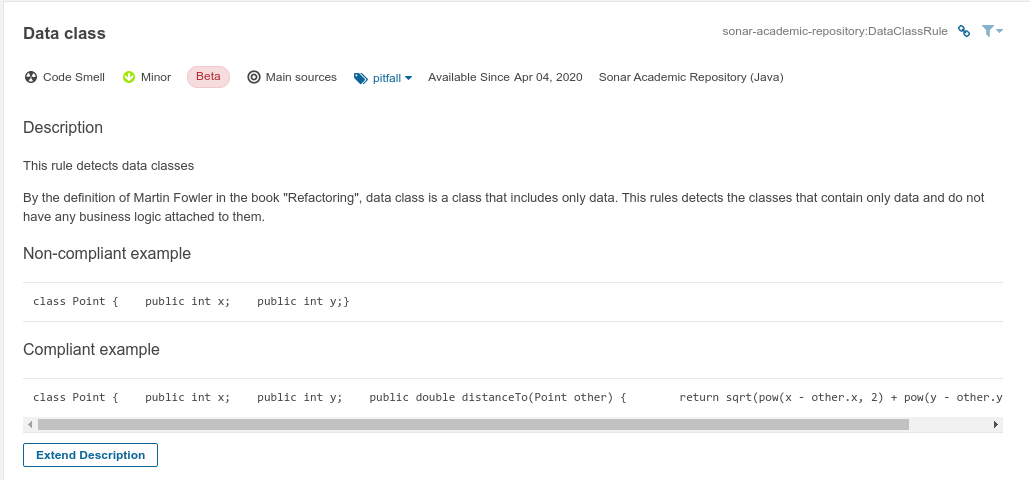
\includegraphics[scale=0.45]{figures/sonarqube_description.png}
    \caption{SonarQube rule description example.}
    \label{fig:sonarqube_description_example}
\end{figure}

Currently, we assume that the user is familiar with the rules and does not require any assistance in understanding how
a given rule works, but it would still be nice to have complete and concise descriptions about rule implementations.

Finally, there as an issue with threshold calculation that has been mentioned in section~\ref{subsec:analysis-results}.
As we did not calculate some thresholds by ourselves, they might be drastically different for Java applications from
Swift applications.

\FloatBarrier

\subsection{Comparison to published results}\label{subsec:comparison-to-published-results}

\TODO {
    Talk about the analysis results:
    \begin{itemize}
        \item Compare with another paper
        \item Take only code smells that are only in that table and compare their and results (paretto chart) (guess the values)
        \item Ignore the blue one (because this is desktop)
        \item It would be nice if the results are not that different (gives some confidence that our calculations make sense), but we can analyze much more
    \end{itemize}
}

In section~\ref{sec:results} we introduced the results that we collected when analyzing our own corpus
of the applications.
Previously, \citeauthor{mannan2016understanding} in~\cite{mannan2016understanding} also investigated code smells in
Android applications.
The main reason why we want to compare the tool described in this paper to the tool used in~\cite{mannan2016understanding}
is that the tool used in that paper is no longer available.
As it was closed-source, commercial solution for code smell analysis, we would like to know how our implementation
compares to the one in~\cite{mannan2016understanding}.

As~\citeauthor{mannan2016understanding} did not provide any concrete distribution of the detected
code smells inside analyzed applications, we had to rely on figure 2 in~\cite{mannan2016understanding} in order
to get the values that collected as a result of the analysis.
Table~\ref{tab:understading_andoid_smells_values} shows the values that we were able to extract from the figure which we used for comparison
with our results.
The figure contains two datasets (\say{mobile} and \say{desktop} applications) and we used the values for the \say{mobile}
dataset, since we were analyzing applications for the Android platform.

\begin{table}
    \begin{center}
        \begin{tabular} {| c | c |}
            \hline
            \textbf{Code smell name} & \textbf{Percentage of occurrence (\%)} \\ \hline
            Data class & 18 \\ \hline
            Data clump & 15.5 \\ \hline
            Cyclic dependencies & 13 \\ \hline
            Feature envy & 9.5 \\ \hline
            External duplication & 9 \\ \hline
            SAPBreaker & 9 \\ \hline
            God class & 5.5 \\ \hline
            Sibling duplication & 4.5 \\ \hline
            Divergent change & 4 \\ \hline
            Message chains & 2.5 \\ \hline
            Intensive coupling & 2.4 \\ \hline
            Tradition breaker & 2 \\ \hline
            Unstable dependencies & 1.75 \\ \hline
            Refused bequest & 1.5 \\ \hline
            Blob class & 1 \\ \hline
            Shotgun surgery & 0.5 \\ \hline
            Internal duplication & 0.25 \\ \hline
        \end{tabular}
        \caption{Distribution of detected code smells from~\cite{mannan2016understanding}.}
        \label{tab:understading_andoid_smells_values}
    \end{center}
\end{table}

As in our paper we analyzed more than the code smells than in~\cite{mannan2016understanding}, we had to normalize
our results so that we could compare the distribution only of those code smells that are present in~\cite{mannan2016understanding}.
Table~\ref{tab:sonar_academic_plugin_values} shows normalized distribution of the code smells (only the ones that
are present in~\cite{mannan2016understanding}).

\begin{table}
    \begin{center}
        \begin{tabular} {| c | c |}
            \hline
            \textbf{Code smell name} & \textbf{Percentage of the occurrence (\%)} \\ \hline
            Data class & 14.7854994 \\ \hline
            Data clump & 5.32531265 \\ \hline
            Cyclic dependencies & 0.54297926 \\ \hline
            Feature envy & 12.69273389 \\ \hline
            SAPBreaker & 16.37011240 \\ \hline
            God class & 3.07424410 \\ \hline
            Divergent change & 48.62751306 \\ \hline
            Message chains & 1.24267849 \\ \hline
            Intensive coupling & 5.06252968 \\ \hline
            Tradition breaker & 0.02691151 \\ \hline
            Unstable dependencies & 0.17255026 \\ \hline
            Refused bequest & 0.50498654 \\ \hline
            Blob class & 0.66170651 \\ \hline
            Shotgun surgery & 4.21719171 \\ \hline
        \end{tabular}
        \caption{Distribution of selected code smells for this paper.}
        \label{tab:sonar_academic_plugin_values}
    \end{center}
\end{table}

Comparison of distributions of both papers can be seen in figure~\ref{fig:comparison_of_distributions}.
It is important to note that we left some of the code smells out of the comparison.
The reason is that we did not implement those rules in our plugin, as those are already natively
supported by SonarQube.
The rules that we excluded from the comparison are \say{external duplication}, \say{sibling duplication} and
\say{internal duplication}.


From this comparison we can see that the number of detections for some code smells is pretty similar and quite different for others.
For instance, the number of detections for \say{blob class} and \say{feature envy} is pretty similar, while
\say{data class} and \say{divergent change} are quite different.

There are multiple reasons why the results are different but here are the ideas on why the difference more noticeable in
some occasions than others.

\begin{flushleft}
    \textbf{Implementation might be different}.
    This means that the code smell definitions in~\cite{mannan2016understanding} might be different from our definition and
    thus we are detecting different things or detecting the same things differently.
    Since the tool from~\cite{mannan2016understanding} is close-source then we are not able to compare the implementations.
\end{flushleft}

\begin{flushleft}
    \textbf{Corpuses are different}.
    The source datasets were not provided by~\citeauthor{mannan2016understanding}, so we are not able to verify our tool against
    the same dataset.
    If we used the same dataset, the results might have been more similar or, on the contrary, different.
\end{flushleft}

\begin{figure} [htb]
    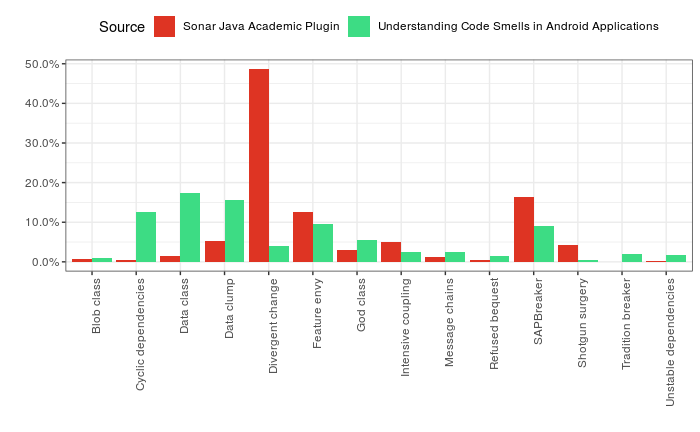
\includegraphics[scale=0.8]{figures/comparison.png}
    \caption{Distribution of detected code smells in our paper versus~\cite{mannan2016understanding}.}
    \label{fig:comparison_of_distributions}
\end{figure}

As the reader might have noticed, there are various reasons why the results might be different.
Nonetheless, different results on different datasets do not mean that one tool is more useful than the other.
In the next chapter we will look into potential usages of the tool developed by us.

\FloatBarrier

\subsection{Potential usages}\label{subsec:potential-usages}

\TODO{
    In this section, we should describe how external users can use our tool.
    We can focus on 3 groups that we will introduce in introduction.
    Developers, project managers and data scientist?
    For each group, we can write a section and describe how they can use the tool and see useful
    information about the projects.
}

In section~\ref{sec:introduction} we mentioned various roles in software development process who might be interested
in the results of an analysis of a software project.
In the next subsections, we will go over the ways how each of the focus groups can use the plugin.

\subsubsection{Developers}

\TODO{
    Think of how this tool is useful for developers.
    Obviously this is the focus group.
}

\TODO{
    Developers can use this tool for statical analysis of the application they develop.
    Here we can show detailed view of a single code smell, with message line
    and rule description and "ideas" on how to fix the bug in the rule description.
}

Developers are our main target group.
SonarQube also has an ability to be integrated into the IDE and be used from there.
Unfortunately, this requires the premium edition (paid) of SonarQube and we only have access to the community edition (free)
so we are not able to show the screenshots from the IDE\@.
Nonetheless, full information is available on the server side after the analysis has been run in the CI/CD environment.
Figure~\ref{fig:dev_1} shows the information that developer sees when a code smell is reported on the Sonar server side.
In the picture we can see the message that was reported by the static analyzer, when it was first introduced,
the line it occurs on, what is the type of the reported issue (in our case it is \say{code smell}) and severity of the detection.

\begin{figure}
    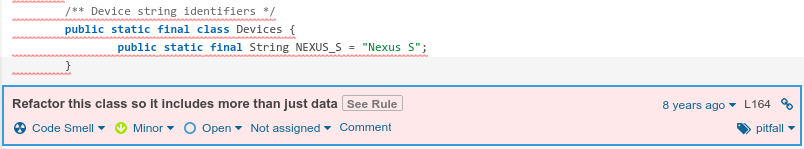
\includegraphics[scale=0.5]{figures/dev_1.png}
    \caption{Example of a reported issue on the server side.}
    \label{fig:dev_1}
\end{figure}

Additionally, developer has an option to press the \say{See rule} button.
When opened, this view shows the description of the reported code smell, as it can be seen in figure~\ref{fig:dev_2}.
This allows the developers to quickly access rule definitions in order to see compliant and non-compliant rule examples.

\begin{figure}
    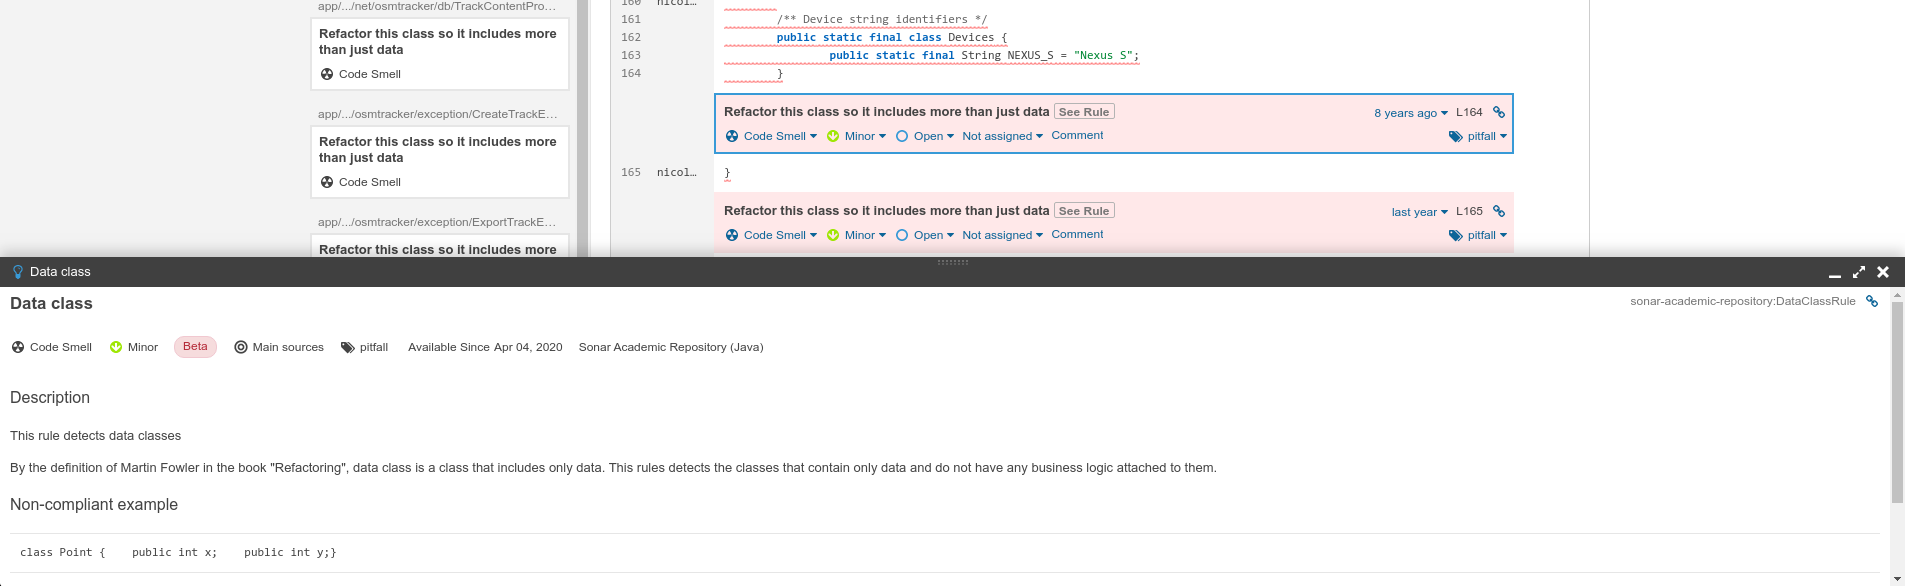
\includegraphics[scale=0.25]{figures/dev_2.png}
    \caption{Example of expanded rule description.}
    \label{fig:dev_2}
\end{figure}

\FloatBarrier

\subsubsection{Project managers}

\TODO{
    Project managers can see the overview of the project and how
    much code smells there are in the project.
    Also they can see how many of each rule, etc.
    Here we can show general view of the project (the dashboard).
}

As mentioned in the previous section, it is possible to integrate the plugin into the IDE.
However, not all the roles in software development are related to coding.
SonarQube provides a nice user interface, that can be useful for project managers to receive an overview of a project,
as seen in figure~\ref{fig:spm_1}.
On this figure we can see different metrics that are helpful to identify the state of the project.
For example, number of bugs, vulnerabilities and code smells detected during static code analysis.

\begin{figure}
    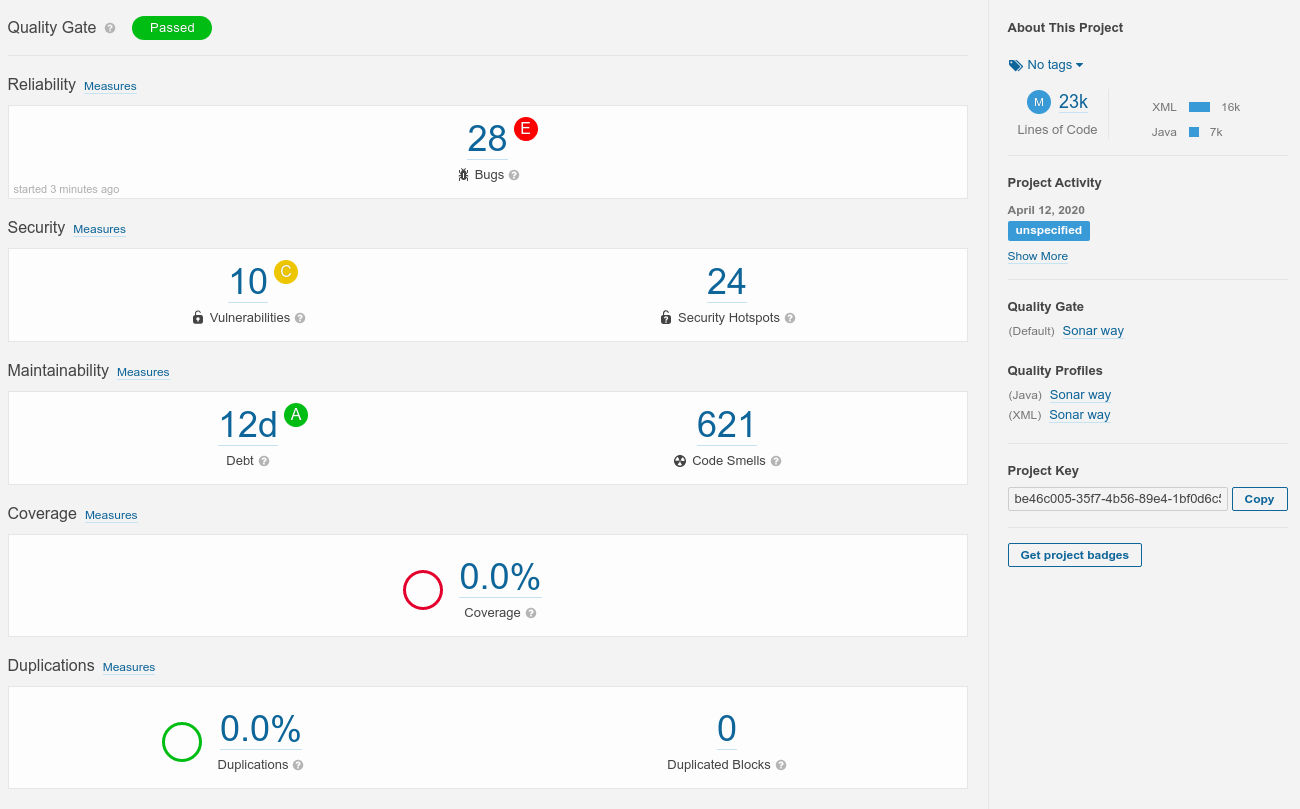
\includegraphics[scale=0.35]{figures/project_managers_1.png}
    \caption{Example of a project overview in the SonarQube user interface.}
    \label{fig:spm_1}
\end{figure}

The view of figure~\ref{fig:spm_1} can be further expanded in order to see more detailed overview of detected
code smells/vulnerabilities as it can be seen in figure~\ref{fig:spm_2}.

\begin{figure}
    \centering
    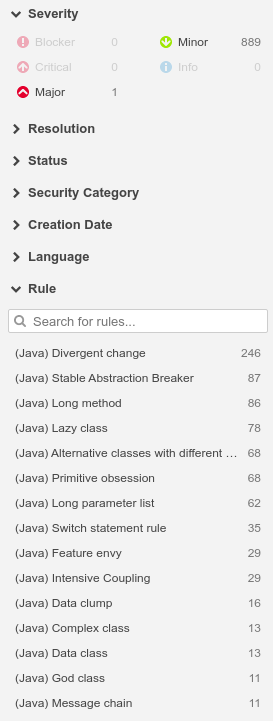
\includegraphics[scale=0.6]{figures/pm_2_1.png}
    \caption{Example of code smell detections grouped by rule.}
    \label{fig:spm_2}
\end{figure}

\FloatBarrier

\subsubsection{Data scientists}

\TODO{
    How can the data scientists use this?
    In general, they can export datasets from SonarQube like we did.
    Perhaps we can describe here how we did this, and what we managed to create (e.g. analysis results).
    With this, they can perhaps find correlations if different code smells can be usually found together.
}

In the era of big data, a lot of useful information can be extracted from the collected data.
Static code analysis is not an exception.
If an organization maintains multiple projects in a SonarQube instance, the data from the static
analysis could be used to find correlations between different code smells in multiple projects.
This could show some trends where certain code smells are popular in multiple teams and could
lead to introduction of new rules in order to fix the code quality issues.

SonarQube provides a rich set of web services that can be used to extract the data into external applications.
The base URI \url{/api/webservices/list} provides description of all webservices exposed by the current SonarQube instance.
For example, the API can be used to export the issues found in the project for further analysis.
In order to achieve this, one would use the \url{/api/issues/search} endpoint in order to search for issues inside the projects.
